\section{Date: 2026-10-03}
\noindent \textbf{Series ID: IM1} 

\noindent This series is titled Import Price Index (SITC): Beverages and tobacco (DISCONTINUED) and has a frequency of Monthly. The units are Index 2000=100 and the seasonal adjustment is Not Seasonally Adjusted.The observation start date is 1995-01-01 and the observation end date is 2005-12-01.The popularity of this series is 1. \\ 

\noindent \textbf{Series ID: A33GUO} 

\noindent This series is titled Manufacturers' Unfilled Orders: Photographic Equipment Manufacturing and has a frequency of Monthly, End of Period. The units are Millions of Dollars and the seasonal adjustment is Seasonally Adjusted.The observation start date is 1992-01-01 and the observation end date is 2026-08-01.The popularity of this series is 1. \\ 

\subsection{Raw Regression}
\noindent Regresses the two series against each other directly. A significant result here can come just as easily from both series sharing a long-run trend as from any real relationship.

\begin{center}
\begin{tabular}{lclc}
\toprule
\textbf{Dep. Variable:}    & value\_fred\_A33GUO & \textbf{  R-squared:         } &     0.048   \\
\textbf{Model:}            &         OLS         & \textbf{  Adj. R-squared:    } &     0.041   \\
\textbf{Method:}           &    Least Squares    & \textbf{  F-statistic:       } &     6.572   \\
\textbf{Date:}             &   Sat, 03 Oct 2026  & \textbf{  Prob (F-statistic):} &   0.0115    \\
\textbf{Time:}             &       15:18:33      & \textbf{  Log-Likelihood:    } &   -929.10   \\
\textbf{No. Observations:} &           132       & \textbf{  AIC:               } &     1862.   \\
\textbf{Df Residuals:}     &           130       & \textbf{  BIC:               } &     1868.   \\
\textbf{Df Model:}         &             1       & \textbf{                     } &             \\
\textbf{Covariance Type:}  &      nonrobust      & \textbf{                     } &             \\
\bottomrule
\end{tabular}
\begin{tabular}{lcccccc}
                          & \textbf{coef} & \textbf{std err} & \textbf{t} & \textbf{P$> |$t$|$} & \textbf{[0.025} & \textbf{0.975]}  \\
\midrule
\textbf{const}            &     -61.5812  &      429.804     &    -0.143  &         0.886        &     -911.897    &      788.734     \\
\textbf{value\_fred\_IM1} &      11.0522  &        4.311     &     2.564  &         0.011        &        2.523    &       19.582     \\
\bottomrule
\end{tabular}
\begin{tabular}{lclc}
\textbf{Omnibus:}       &  1.052 & \textbf{  Durbin-Watson:     } &    0.033  \\
\textbf{Prob(Omnibus):} &  0.591 & \textbf{  Jarque-Bera (JB):  } &    0.646  \\
\textbf{Skew:}          &  0.122 & \textbf{  Prob(JB):          } &    0.724  \\
\textbf{Kurtosis:}      &  3.241 & \textbf{  Cond. No.          } & 1.77e+03  \\
\bottomrule
\end{tabular}
%\caption{OLS Regression Results}
\end{center}

Notes: \newline
 [1] Standard Errors assume that the covariance matrix of the errors is correctly specified. \newline
 [2] The condition number is large, 1.77e+03. This might indicate that there are \newline
 strong multicollinearity or other numerical problems.

\begin{figure}
\centering
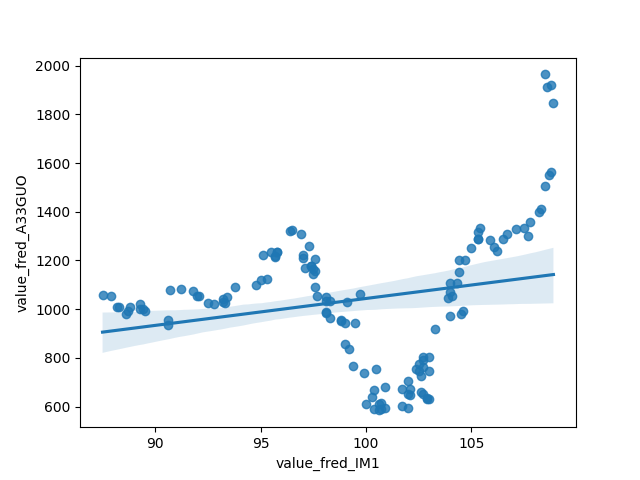
\includegraphics[scale = 0.9]{plots/plot_2026-10-03.png}
\caption{Raw Regression Plot for 2026-10-03}
\end{figure}
\newpage
\subsection{Detrended Regression}
\noindent Regresses the residuals of each series after removing its own linear time trend, so a shared trend can no longer drive the result on its own. A relationship that stays significant here is better evidence of a genuine link between the two series.

\begin{center}
\begin{tabular}{lclc}
\toprule
\textbf{Dep. Variable:}              & value\_fred\_A33GUO\_detrended & \textbf{  R-squared:         } &     0.001   \\
\textbf{Model:}                      &              OLS               & \textbf{  Adj. R-squared:    } &    -0.007   \\
\textbf{Method:}                     &         Least Squares          & \textbf{  F-statistic:       } &   0.09245   \\
\textbf{Date:}                       &        Sat, 03 Oct 2026        & \textbf{  Prob (F-statistic):} &    0.762    \\
\textbf{Time:}                       &            15:18:33            & \textbf{  Log-Likelihood:    } &   -929.09   \\
\textbf{No. Observations:}           &                132             & \textbf{  AIC:               } &     1862.   \\
\textbf{Df Residuals:}               &                130             & \textbf{  BIC:               } &     1868.   \\
\textbf{Df Model:}                   &                  1             & \textbf{                     } &             \\
\textbf{Covariance Type:}            &           nonrobust            & \textbf{                     } &             \\
\bottomrule
\end{tabular}
\begin{tabular}{lcccccc}
                                     & \textbf{coef} & \textbf{std err} & \textbf{t} & \textbf{P$> |$t$|$} & \textbf{[0.025} & \textbf{0.975]}  \\
\midrule
\textbf{const}                       &   -1.762e-10  &       24.188     & -7.28e-12  &         1.000        &      -47.854    &       47.854     \\
\textbf{value\_fred\_IM1\_detrended} &       7.4297  &       24.436     &     0.304  &         0.762        &      -40.913    &       55.773     \\
\bottomrule
\end{tabular}
\begin{tabular}{lclc}
\textbf{Omnibus:}       &  1.009 & \textbf{  Durbin-Watson:     } &    0.033  \\
\textbf{Prob(Omnibus):} &  0.604 & \textbf{  Jarque-Bera (JB):  } &    0.617  \\
\textbf{Skew:}          &  0.125 & \textbf{  Prob(JB):          } &    0.735  \\
\textbf{Kurtosis:}      &  3.223 & \textbf{  Cond. No.          } &     1.01  \\
\bottomrule
\end{tabular}
%\caption{OLS Regression Results}
\end{center}

Notes: \newline
 [1] Standard Errors assume that the covariance matrix of the errors is correctly specified.

\begin{figure}
\centering
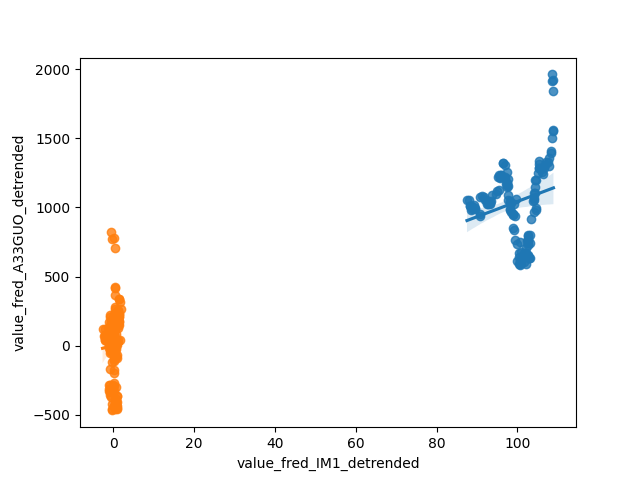
\includegraphics[scale = 0.9]{plots/plot_2026-10-03_detrended.png}
\caption{Detrended Regression Plot for 2026-10-03}
\end{figure}
\newpage
